\section{Reducing Overheads of Run-Time Monitoring}
\label{sec:optimizations}

% Overview of overhead vs. coverage space
\begin{figure}
  \begin{center}
    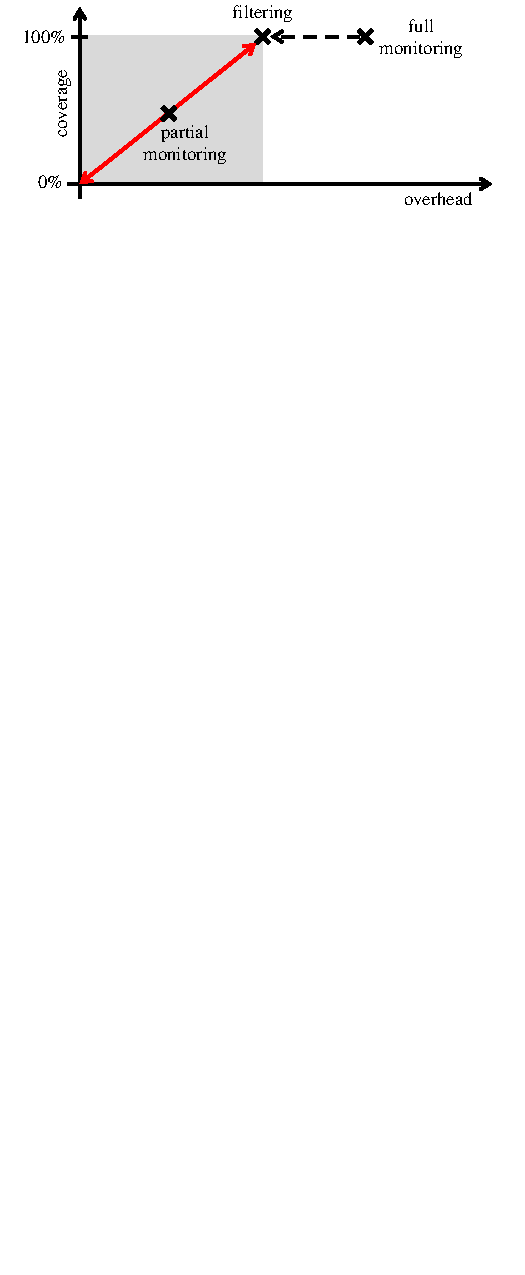
\includegraphics[width=\columnwidth]{figs/optimization_overview.pdf}
    \vspace{-0.2in}
    \caption{Filtering can be used to reduce the overheads. Partial monitoring
    allows a further trade-off between coverage and overheads.}
    \label{fig:optimizations.overview}
    \vspace{-0.1in}
  \end{center}
\end{figure}

The overheads of monitoring can be high. Figure~\ref{dummy} shows the full
monitoring overheads for three example monitoring extensions: array bounds
check (BC), uninitialized memory check (UMC), and dynamic information flow
tracking (DIFT). In order to reduce these overheads, we present two
optimizations. The first is to filter out monitoring events which relate to
null metadata (Section~\ref{sec:optimizations.filter}). Second, in order to
further reduce overheads, we propose to trade-off monitoring coverage. By
performing partial monitoring, we can further decrease the overheads incurred
due to monitoring. Figure~\ref{fig:optimizations.overview} shows an overview of
these ideas. Filtering allows us to reduce the overheads of monitoring and
partial monitoring allows us to further reduce overheads and create a trade-off
between overheads and coverage.

\subsection{Filtering Null Metadata Events}
\label{sec:optimizations.filter}

The instruction-grained run-time monitoring schemes we focus on typically set
and keep track of metadata information. This metadata information is used to
verify security or reliability probabilities. For example, for array bounds
check, the monitoring core stores metadata describing the base and bounds
addresses for array pointers. This metadata is checked on load and store
instructions. If the metadata for an event is null, then it is not relevant to
array bounds check since this represents a non-array pointer object. By
filtering out these null monitoring events, we can reduce the overheads of
monitoring by reducing the amount of work the monitoring core must do.

In order to filter out null monitoring events, we need an efficient method to
keep track of which events are null. In addition, when we filter out a null
monitoring event, we must ensure that any metadata updates that were skipped
are handled properly. Typically, these null monitoring events are just
propagating this null metadata information. Thus, when we filter out one of
these events, we must ensure that the destination operand is marked as null. In
other words, we need to be able to track the dataflow for these null metadata.

\subsection{Trading-Off Coverage for Reduced Overheads}
\label{sec:optimizations.drop}

There is a limit to the reduction in overheads by using filtering. We propose
that overheads can be further reduced by performing partial monitoring. As the
monitoring schemes we target consist of a large number of independent
monitoring checks, it can still be possible to provide partial protection by
performing a portion of the monitoring operations. Thus, we aim to enable this
trade-off between overheads and monitoring coverage.

The high-level idea is to track the run-time monitoring overheads. When the
overhead exceeds our target overhead, we will drop monitoring operations.  Of
course, dropping monitoring operations implies that some functionality of the
monitoring scheme has been lost.  This may cause either false negatives, where
an error that occurs in the main program's execution is not detected, or false
positives, where the monitor incorrectly believes an error has occurred.  For
example, a false positive can occur for array bounds check if an event is
dropped that handles copying a pointer. A subsequent array access using the new
pointer will incorrectly cause an error to be raised since the new pointer's
base and bounds will not be correctly set.  We accept false negatives as the
loss in coverage that we trade off in order to limit overheads.  However, we
must safely drop monitoring events in such a way as to avoid false positives so
that the system does not incorrectly raise an error.

In analyzing various monitoring schemes, we found that monitoring operations
are primarily of two types: \emph{checks} and \emph{metadata updates}. Monitors
\emph{check} certain properties to ensure correct main program execution and
they \emph{update} metadata for bookkeeping. Skipping a check operation can
only cause false negatives and will never cause a false positive. Therefore, we
may simply skip a check operation. Skipping an update operation can cause false
negatives but may also cause false positives. Essentially, when an update
operation is skipped, we can no longer trust the corresponding metadata. Thus,
we need to be able to mark these invalid metadata. Furthermore, metadata that
would be derived from these dropped events also will be invalid. In other
words, we need to be able to track the dataflow of invalid metadata when
monitoring operations are dropped.
